\chapter{Divide Areas Algorithm}
\label{chp:DARP}
In this project, the distributed method of multi-robot coverage path planning is implemented. Several different algorithms of this type are discussed in Section \ref{sec:lit Ditributed MCPP}. The algorithm being discussed in this chapter is briefly addressed in Section \ref{subsec:lit DARP}. Section \ref{sec:DARP bg} addresses \ac{darp} in more detail, and Section \ref{sec:DARP dist} discusses the implementation of the algorithm with different distance measures. Section \ref{sec:DARP implement} then goes on to show the implementation of DARP in different practical scenarios. 
% TODO: review section breakdown
\section{Background Theory}
\label{sec:DARP bg}
Grid-based coverage path planning can be implemented using a number of different methods. % TODO: Refer back to literature review

Naturally, achieving the most optimal solution possible would be most desirable. The authors of \cite{DARP2017} propose a set of requirements for optimal coverage path planning using a grid-based approach. These fundamental conditions, as they call them, are listed below.
\begin{enumerate}
	\item Every cell in the environment, that is not classified as an object, must be covered. This is known as complete coverage.
	\item Each cell in the environment must only be searched once, and only by one of the robots. This is known as the non-backtracking requirement.
	\item Each robot should have as close to an equal amount of cells as possible assigned to it for searching. Their sets of cells should be of roughly the same size.
	\item The sets of cells assigned to each robot should be a connected sub-region. This means that when generating a path to search the cells within its set, a robot would not need to traverse that of another to search it's own sub-region.
	\item The initial position of each robot should be contained within the set of cells assigned to it. This means that a robot would not need to traverse another robot's sub-region to reach its sub-region for searching.
\end{enumerate}
The authors developed a methodology to achieve these optimal conditions. They called it The \ac{darp}. Their solution seeks to divide a known environment containing static obstacles into contiguous sub-regions. These regions are formed based on the robot starting positions so that each robot starts within one of the regions.

The solution is found in an iterative manner and it converges to where the sub-regions are cohesive and roughly the same size. \ac{darp} only divides the environment appropriately between robots. A single robot \ac{cpp} algorithm can then be utilized to achieve complete coverage of each sub-region, which translates to complete coverage of the whole environment.

% Distributed - justification
This is a distributed method, which means that each robot travels only within its sub-region. These regions don't overlap, meaning that the robots will never collide, provided they follow their planned path. Therefore, it removes a layer of complexity that generally gets added with multi-robot approaches. 

% Offline
It is also an offline approach to \ac{cpp}, so the environment is known prior to the planning phase. This phase includes the divide areas algorithm and the sub-region coverage algorithm which is discussed in Chapter \ref{chp:Subregion-Coverage}. 
% TODO: Maybe mention something about the EXISTENCE of solutions
\subsection{Algorithm Description}
The algorithm works on a two-dimensional environment that is divided into discrete cells. Once the discretisation is complete, the algorithm starts by operating similar to a Voronoi partition. It constructs a matrix for each robot with the same dimension as the environment. The authors refer to these as the Evaluation Matrices ($E_i$). They contain the distances from each cell in the environment to the respective robots. Euclidean distance was used as the distance measure.
\begin{figure}[h!]
	\centering
	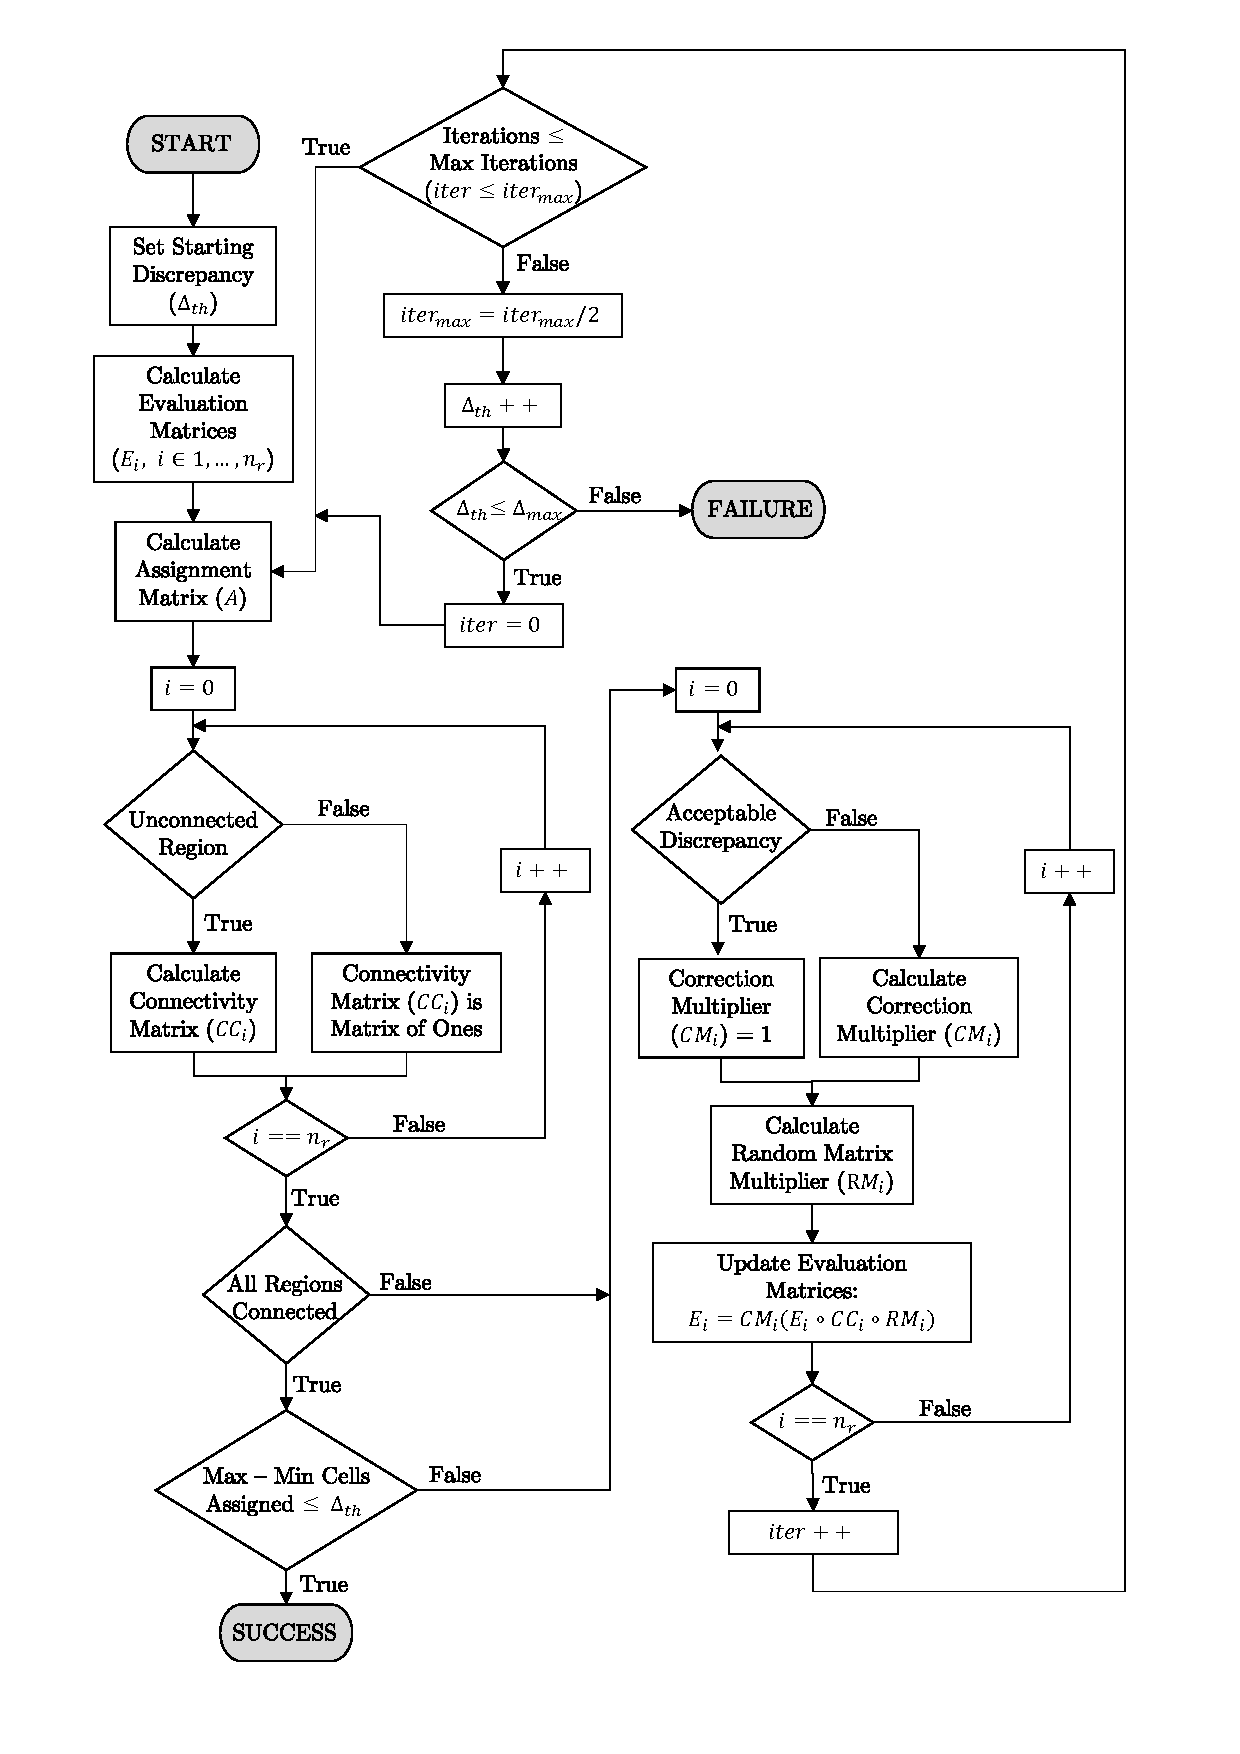
\includegraphics[scale=0.8,trim={1.5cm 0 1.5cm 0},clip]{figs/DARP_Diagram3.pdf}
	\caption{Flow diagram representing the logic for DARP.}
	\label{fig:DARP}
\end{figure}

\section{Distance Measure Comparisons}
\label{sec:DARP dist}
% Include thing where you compare distance measures and how it effects number of iterations

\section{Implementation with Different Scenarios}
\label{sec:DARP implement}
% Different Environments, Obstacle Dispersion and Robot Dispersion